\let\negmedspace\undefined
\let\negthickspace\undefined
\documentclass[journal]{IEEEtran}
\usepackage[a5paper, margin=10mm, onecolumn]{geometry}
%\usepackage{lmodern} % Ensure lmodern is loaded for pdflatex
\usepackage{tfrupee} % Include tfrupee package

\setlength{\headheight}{1cm} % Set the height of the header box
\setlength{\headsep}{0mm}     % Set the distance between the header box and the top of the text

\usepackage{gvv-book}
\usepackage{gvv}
\usepackage{cite}
\usepackage{amsmath,amssymb,amsfonts,amsthm}
\usepackage{algorithmic}
\usepackage{graphicx}
\usepackage{textcomp}
\usepackage{xcolor}
\usepackage{txfonts}
\usepackage{listings}
\usepackage{enumitem}
\usepackage{mathtools}
\usepackage{gensymb}
\usepackage{comment}
\usepackage[breaklinks=true]{hyperref}
\usepackage{tkz-euclide} 
\usepackage{listings}
% \usepackage{gvv}                                        
\def\inputGnumericTable{}                                 
\usepackage[latin1]{inputenc}                                
\usepackage{color}                                            
\usepackage{array}                                            
\usepackage{longtable}                                       
\usepackage{calc}                                             
\usepackage{multirow}                                         
\usepackage{hhline}                                           
\usepackage{ifthen}                                           
\usepackage{lscape}
\begin{document}

\bibliographystyle{IEEEtran}
\vspace{3cm}

\title{2.9.16}
\author{EE25BTECH11065 - Yoshita}
% \maketitle
% \newpage
% \bigskip
{\let\newpage\relax\maketitle}

\renewcommand{\thefigure}{\theenumi}
\renewcommand{\thetable}{\theenumi}
\setlength{\intextsep}{10pt} % Space between text and floats

\textbf{Question}:\\
Prove that three points A, B, and C with position vectors $\mathbf{a}$, $\mathbf{b}$, and $\mathbf{c}$ respectively are collinear if and only if $(\mathbf{b} \times \mathbf{c}) + (\mathbf{c} \times \mathbf{a}) + (\mathbf{a} \times \mathbf{b}) = \mathbf{0}$.\\
\bigskip

\textbf{Solution}:\\
The three points A, B, and C are collinear if and only if the vectors $\vec{AB}$ and $\vec{AC}$ are parallel. The position vectors for these are:
\begin{table}[H]    
  \centering
  \begin{tabular}{|c|c|}
\hline
\textbf{Name} & \textbf{Value} \\ \hline
$\vec{A}$ & $\myvec{2 & 1 \\0 & 3}$ \\ \hline
\end{tabular}

  \caption{Answers}
  \label{Answers}
\end{table}
\begin{align*}
    \mathbf{A-B} &= \vec{b} - \vec{a} \\
    \mathbf{A-C} &= \vec{c} - \vec{a}
\end{align*}
If two vectors are collinear,
\begin{align}
    (\mathbf{b} - \mathbf{a}) \times (\mathbf{c} - \mathbf{a}) &= \mathbf{0}
\end{align}
Using the determinant (matrix) form of the cross product,

\[
(\mathbf{b}-\mathbf{a}) \times (\mathbf{c}-\mathbf{a}) =
\begin{vmatrix}
\mathbf{i} & \mathbf{j} & \mathbf{k} \\
\myvec{b_1-a_1} & \myvec{b_2-a_2} & \myvec{b_3-a_3} \\
\myvec{c_1-a_1} & \myvec{c_2-a_2} & \myvec{c_3-a_3}
\end{vmatrix}
\]
Rearranging the equation we get,
\begin{align}
    (\mathbf{a} \times \mathbf{b}) + (\mathbf{b} \times \mathbf{c}) + (\mathbf{c} \times \mathbf{a}) &= \mathbf{0}
\end{align}
Hence we proved that that three points A, B, and C with position vectors $\mathbf{a}$, $\mathbf{b}$, and $\mathbf{c}$ respectively are collinear if and only if $(\mathbf{b} \times \mathbf{c}) + (\mathbf{c} \times \mathbf{a}) + (\mathbf{a} \times \mathbf{b}) = \mathbf{0}$
\begin{figure}[h!]
\begin{center}
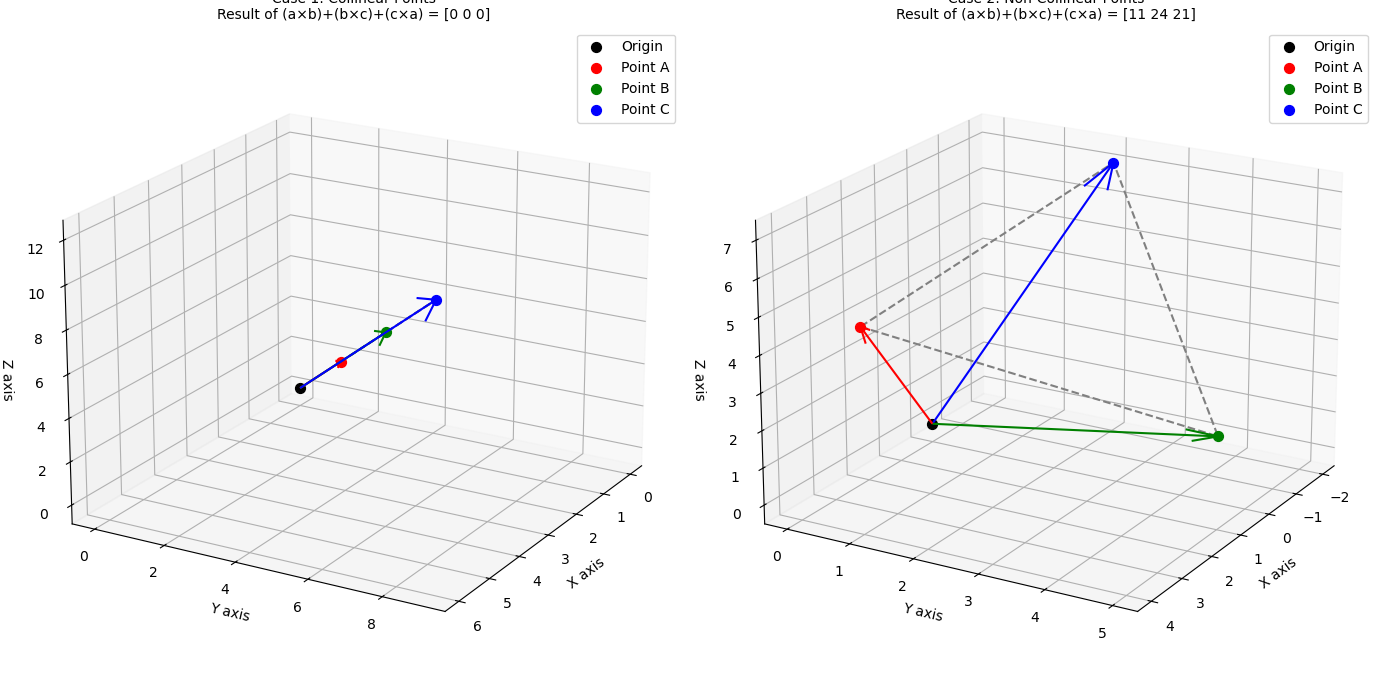
\includegraphics[width=0.9\columnwidth]{figs/fig1.png}
\end{center}
\caption{}
\label{fig:Fig.1}
\end{figure}
\end{document}
